\documentclass[12pt,a4paper]{scrartcl}
\usepackage[utf8x]{inputenc}
\usepackage{ucs}
\usepackage[german]{babel}
\usepackage{textcomp}
\usepackage{graphicx}
\usepackage{wrapfig} %Grafiken von Text umfliessen lassen
\usepackage{multicol} %zweispaltiger Text
\usepackage{multirow} %mehrere Tabellenzeilen zu einer zusammenfassen
\usepackage{rotating} %Rotation von Schrift
\usepackage{wallpaper} %Bilder auch ans Hintergrundbilder einbinden
\usepackage{hyperref} %Um in der PDF-Version klickbare Hyperlinks zu haben
\usepackage{color} % für Farben im allgemeinen
\usepackage{colortbl} %farbige Tabellen
\usepackage[final]{pdfpages}
\usepackage[a4paper,left=15mm,right=15mm, top=12mm, bottom=26mm]{geometry} %Seitenränder
\usepackage{paralist}

\makeatletter
\providecommand*{\input@path}{{..}}
\g@addto@macro\input@path{{../}}% append % if you cant override it
\graphicspath{{../}}

\makeatother

\newcommand*\Newpage{\newpage\null\thispagestyle{empty}\newpage}

% Load any packages needed for this document
\begin{document}

\newpage
\section{Mini Don't Panic}
\subsection*{Ein Stundenplan zum Ausfüllen}
\newcommand{\x}{\parbox[0pt][2.7cm][c]{3.7cm}{\hspace{3.7cm}} }
\newcommand{\xT}{\parbox[0pt][1.6cm][c]{1.9cm}{\hspace{3.7cm}} }
% --- Farbdefinitionen ----------------------------------------
\definecolor{hellgrau}{rgb}{0.95,0.95,0.95}

%\begin{sidewaystable}
%\begin{addmargin}[-2mm]{0cm}

%\begin{center}
%\begin{tabular}{|c|c|c|c|c|c|}
%\hline Zeit & Montag & Dienstag & Mittwoch & Donnerstag & Freitag \\
%\hline 8-10  & \x & \x & \x & \x & \x \\
%\hline 10-12 & \x & \x & \x & \x & \x \\
%\hline 12-14 & \x & \x & \x & \x & \x \\
%\hline 14-16 & \x & \x & \x & \x & \x \\
%\hline 16-18 & \x & \x & \x & \footnotesize 16:00 : Fachschaftstreffen & \x \\
%\hline ab 18 & \x & \x & \x & \x & \x \\
%\hline
%\end{tabular}
%\end{center}

%\end{addmargin}
%\end{sidewaystable}

\vspace{23.6cm} % ein Korrekturabstand wg. Drehen
\begin{center}
\begin{rotate}{90}
\begin{tabular}{|c|c|c|c|c|c|}
\hline \cellcolor{black} \xT
	& \cellcolor{black} \textcolor{white}{\textbf{Montag}}
	& \cellcolor{black} \textcolor{white}{\textbf{Dienstag}}
	& \cellcolor{black} \textcolor{white}{\textbf{Mittwoch}}
	& \cellcolor{black} \textcolor{white}{\textbf{Donnerstag}}
	& \cellcolor{black} \textcolor{white}{\textbf{Freitag}} \\
\hline 8:00-10:00  & \x & \x & \x & \x & \x \\
\hline  \cellcolor{hellgrau}10:00-12:00 &  \cellcolor{hellgrau} \x &  \cellcolor{hellgrau} \x &  \cellcolor{hellgrau} \x &  \cellcolor{hellgrau} \x &  \cellcolor{hellgrau} \x \\
\hline 12:00-14:00 & \x & \x & \x & \x & \x \\
\hline  \cellcolor{hellgrau} 14:00-16:00 &  \cellcolor{hellgrau} \x &  \cellcolor{hellgrau} \x &  \cellcolor{hellgrau} \x &  \cellcolor{hellgrau} \x &  \cellcolor{hellgrau} \x \\
\hline 16:00-18:00 & \x & \x & \x & \footnotesize & \x \\
\hline  \cellcolor{hellgrau} 18:00-20:00 &  \cellcolor{hellgrau} \x &  \cellcolor{hellgrau} \x &  \cellcolor{hellgrau} \x &  \cellcolor{hellgrau} \x &  \cellcolor{hellgrau} \x \\
\hline
\end{tabular}
\end{rotate}
\end{center}

\newpage

\begin{sidewaysfigure}
    \centering
    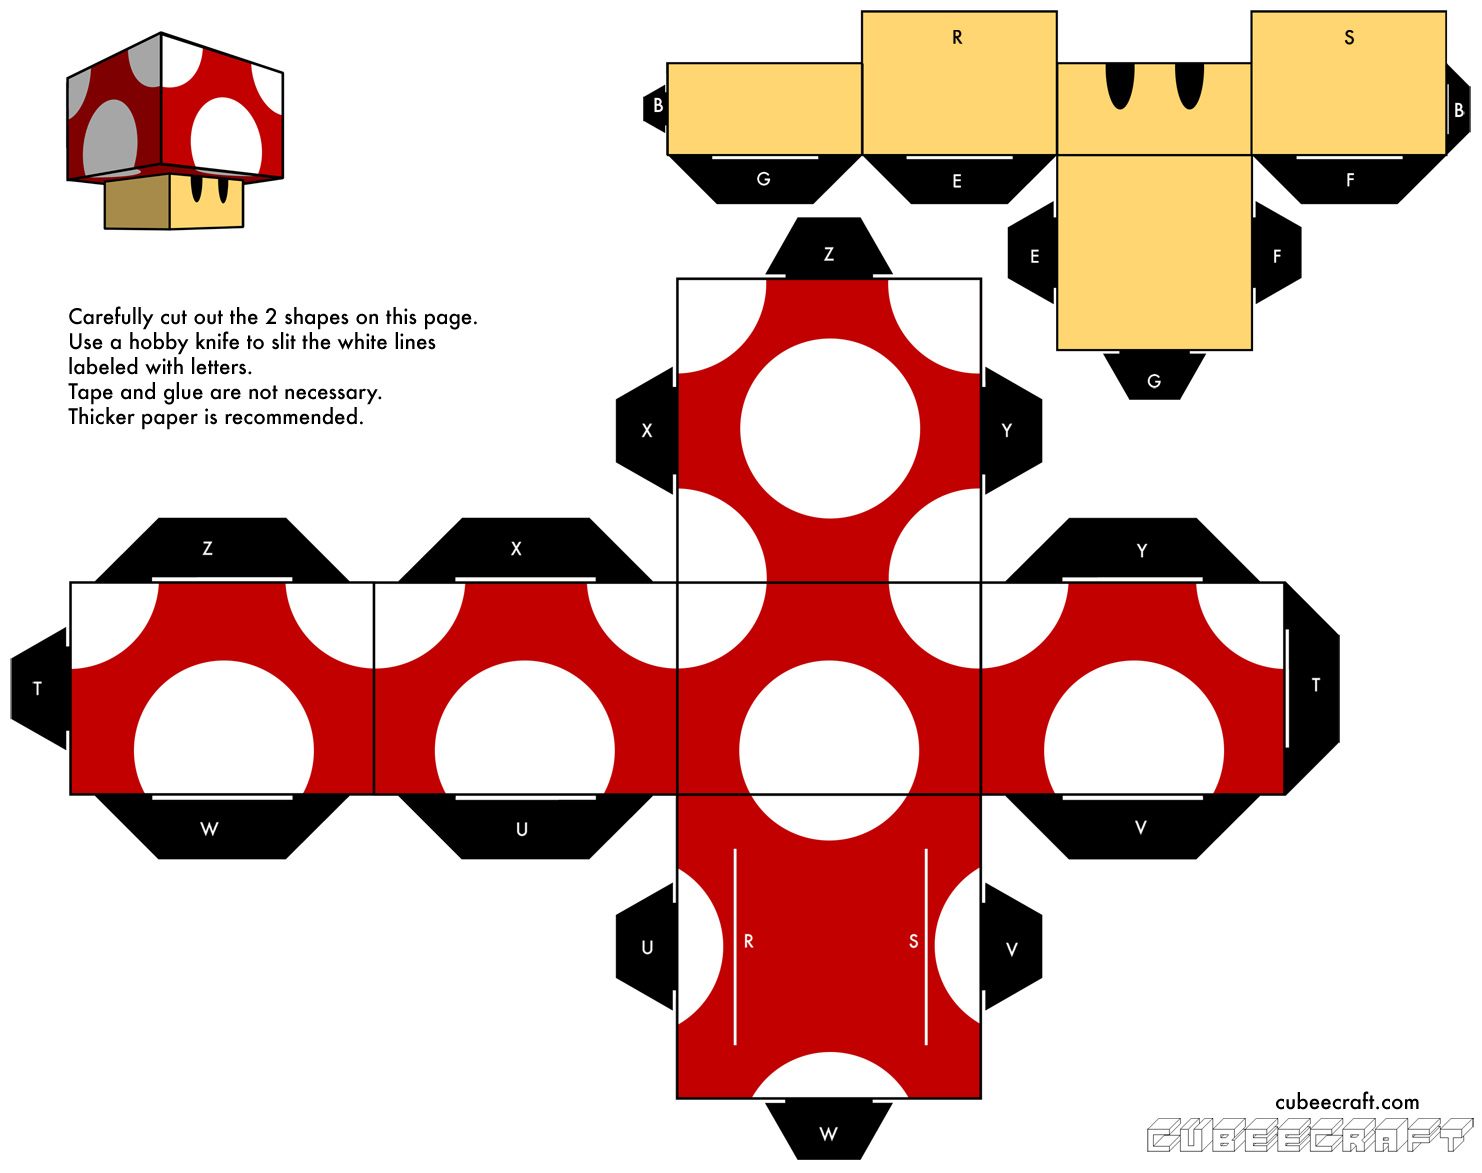
\includegraphics[scale=1]{bilder/Cubeecraft_Mushroom_Super_mario.jpg}
\end{sidewaysfigure}

%\begin{sidewaysfigure}
%    \centering
%    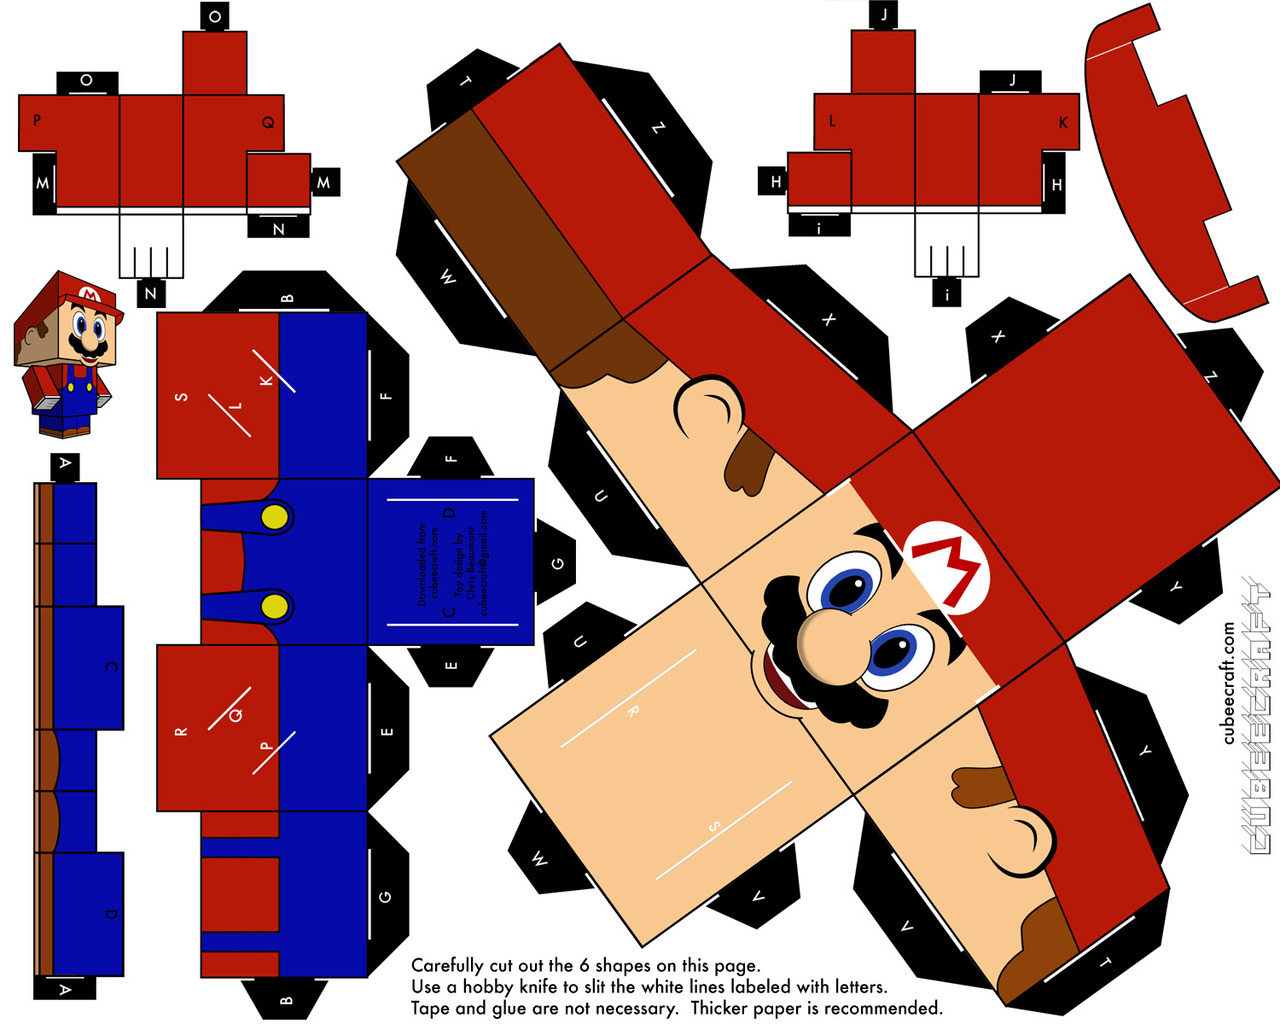
\includegraphics[scale=1]{bilder/super_mario_papercraft.jpg}
%\end{sidewaysfigure}

\newpage

\subsection*{Wo ist was?}
    		\subsubsection{Bockenheim}
			Wichtig für die Vorlesungen und Übungen:\\
			\fbox{
			\begin{tabular}{rrl}
				Hörsäle: & H 1 - H 16  & Teil des Hörsaalgebäudes über dem Cafe.\\
				{} & H I - H VI  & Andere Teil des Hörsaalgebäudes, welcher nicht\\
				{} & {} & über dem Cafe ist.\\
				{} & Magnushörsaal & In der Informatik\\
				{} & {} & {}\\
				Seminarräume: & SR9, SR11 & Informatik EG\\
				{} & 307 & Informatik 3.Stock\\
				{} & NM...& Diese Räume sind in der neuen Mensa\\
				{} & \multicolumn{2}{l}{Alle anderen dreistellingen Zahlen sind im Matheturm}\\
			\end{tabular}}
			\ \\\\ 
			Sonstige Interessante Orte:\\
			\fbox{
				\begin{tabular}{rp{11cm}}
					Cafe Struwwelpeter: & Hier gib es Getränke und kaltes Essen. Du findest es im\\
					{} & Hörsaalgebäude.\\
					Cafeteria: & Verkauft warme Gerichte und gehört zum Studentwerk.  \\
					{} & Ihr findet die Cafeteria in der neuen Mensa.\\
					Leipziger Straße: & Falls ihr aus gegebenen Anlässen keine Lust mehr auf Mensa essen habt, dann gibt es hier alles was das Herz begehrt(Nicht nur Essen).
				\end{tabular}
			}
		
		\subsubsection{Westend}
			Das Westend ist für euer Studium erst interessant, wenn ihr ein Anwendungsfach der Geisteswissenschaften gewählt habt oder ihr Fragen oder Probleme mit dem HRZ oder der Uni habt. Außerdem ist das Westend ein perfekter Ort für eine Studentensafari. Nirgendwo sonst gibt es einen Lebensraum, wo die Reviere so unterschiedlicher Studenten aufeinander treffen. \\
		
		\subsubsection{Riedberg}
			Genauso wie das Westend, ist der Riedberg erst mit der Wahl eines Anwendungsfaches interessant. Bis auf der Tatsache, dass wir uns von Anfang an dort wohlfühlen.
		\subsubsection{Niederrad und Ginnheim}
			Orte, wo die meisten von uns nie sein werden. In Ginnheim befinden sich die Unisportanlagen und in Niederrad die Medizin.
	


    \clearpage

\subsection*{ It's dangerous to go alone! Take this. }
    \vspace{2.5cm}
    \begin{center}
    \fbox{
    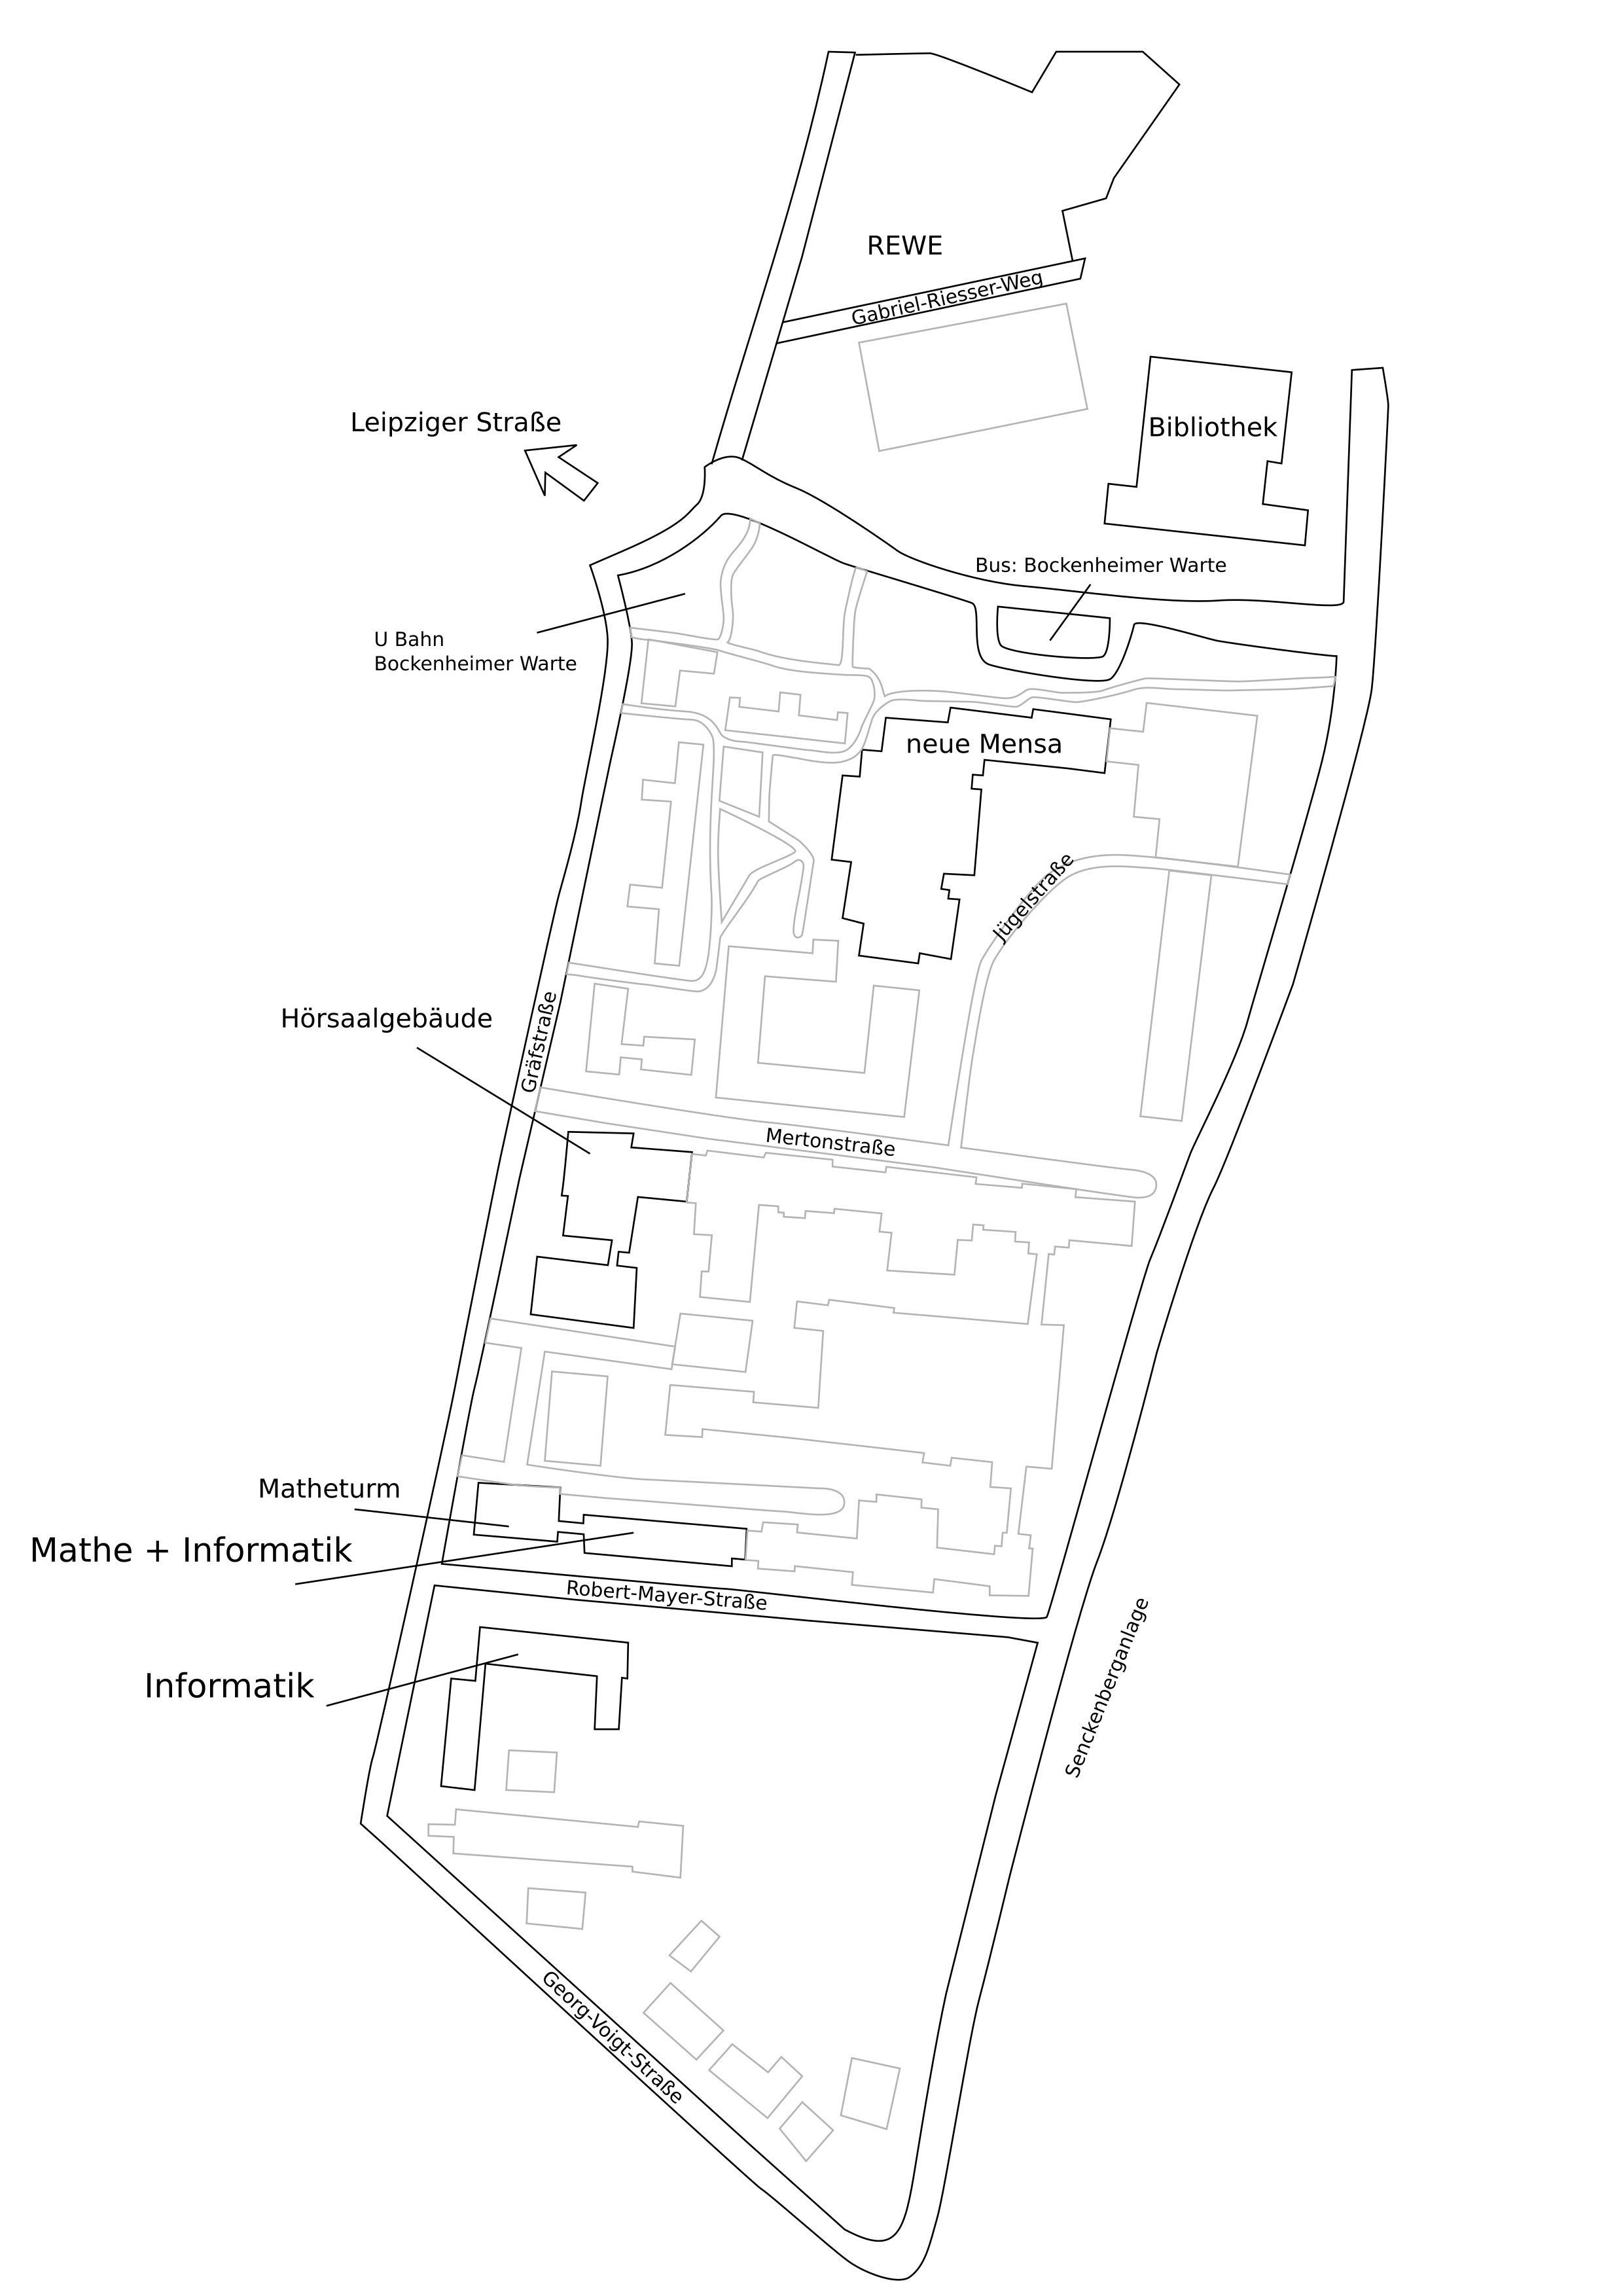
\includegraphics[width=0.8\linewidth]{bilder/KarteB}}
    \\Bockenheim Map
    \end{center}
    \pagebreak

\end{document}
